\section{Graphs}

\subsection{Include Graphs}

\begin{frame}[fragile]{Include Graphs}
Before all, you need the \packagename{graphics} or \packagename{graphicx} package, where \packagename{graphicx} is an extended and enhanced one. So you are recommended to insert the command in the preamble of your document.

\begin{command}
\LC|\usepackage{graphicx}|
\end{command}

Then you can use the command \LC|\includegraphics| to insert images of many formats, including \packagename{jpg}, \packagename{png} images and even other \packagename{pdf} files. \packagename{eps} images should be supported by most modern \LaTeX\ distributions as well.

\begin{command}
\LC|\includegraphics[options]{filename}|
\end{command}

\end{frame}

\begin{frame}[fragile]
There are some example images defined, you can insert them if the figure is not yet ready when writing \LaTeX\ code. They are \packagename{example-image}, \packagename{example-image-golden}, \packagename{example-image-a}, \packagename{example-image-b} and etc.

\begin{latexexample}
\includegraphics[width=0.4\textwidth]{example-image}
\end{latexexample}

We usually use the \packagename{width} option to adjust the size of the image, according to a ratio of \LC|\textwidth|, which means the maximum width of text here.

\end{frame}


\begin{frame}[fragile]{Options of Include Graphs}
	Here some useful \packagename{options} are listed:
	\begin{itemize}
		\item \packagename{height} - use any \LaTeX\ measuring unit.
		\item \packagename{width} - use any \LaTeX\ measuring unit.
		\item \packagename{scale} - scale the graph to this proportion
		\item \packagename{angle} - rotate the graph in anti-clockwise by this angle 
	\end{itemize}
	
	\LaTeX\ measuring unit can be \LC|\textwidth|, \LC|\linewidth|, \LC|\textheight|, \LC|\lineheight|, cm, pt, em, and etc..

\begin{latexexamplesplit}
\includegraphics[width=4cm]%
{example-image-a}
\end{latexexamplesplit}

\end{frame}

\subsection{Figures}

\begin{frame}[fragile]{The \packagename{figure} Environment}
	The \packagename{figure} environment provides a wrapper of image inserted by \LC|\includegraphics|, which add caption and label (reference) to an image. They are especially useful in report and paper writing, here is a template of how to use the environment.

\begin{command}
\begin{LCL}
\begin{figure}[position]
  \centering
  \includegraphics[options]{filename}
  \caption{caption}
  \label{fig:label}
\end{figure}
\end{LCL}
\end{command}
	
\begin{itemize}
			\item \packagename{filename} - the filename or relative path of the graph you want to insert, usually placed in the same or child directory as the tex file
			\item \packagename{position} - we usually use \packagename{!htbp} or \packagename{!H} here, which will be introduced later in this chapter
			\item \packagename{caption} - the caption displayed above/under the graph
			\item \packagename{label} - used for references in a document (will be introduced later)
\end{itemize}

\end{frame}

\begin{frame}[fragile]{Labels and References}

You can use \LC|\ref| to have a reference of a figure by its label. The figures will be automatically numbered (like equations), and the reference is also a hyperlink.

\begin{latexexamplesplit}
\begin{figure}[!htbp]
  \centering
  \includegraphics[
    width=0.7\textwidth,
    angle=90
  ]{example-image-b}
  \caption{Example Image B rotated by 90 degree.}
  \label{fig:img-b}
\end{figure}
B was shown in Figure
\ref{fig:img-b}.
\end{latexexamplesplit}


\end{frame}

\begin{frame}[fragile]{Floats and Positions}

Floats are containers for things in a document that cannot be broken over a page. \LaTeX\ by default recognizes \packagename{figure} and \packagename{table} (will be introduced later) floats. \medskip

If you don't provide the \packagename{position} option, \LaTeX\ will try to help you find a place to set the figure. However, the position is often not ideal, so you need to add some specifiers yourselves. 

\begin{itemize}
\item \packagename{h} - Place the float \structure{here}, i.e., approximately at the same point it occurs in the source text (however, not exactly at the spot)
\item \packagename{t} - Position at the \structure{top} of the page.
\item \packagename{b} - Position at the \structure{bottom} of the page.
\item \packagename{p} - Put on a special \structure{page} for floats only.
\item \packagename{!} - Override internal parameters \LaTeX\ uses for determining ``good'' float positions.
\item \packagename{H} -  Places the float at precisely the location in the \LaTeX\ code. Requires the float package, i.e., \LC|\usepackage{float}|.
\end{itemize}

\end{frame}


\begin{frame}[fragile]{Include Multiple Graphs}
    A useful extension is the \packagename{subcaption} package, which provides a \packagename{subfigure} environment to add multiple subfigures in a figure. \medskip
    
    Note that there is also a package called \packagename{subfigure}, but is has been deprecated (not maintained), please do not use it. Another package called \packagename{subfig} provides the same commands as that of \packagename{subfigure} package. However, they can't be used together. \medskip
    
    In simplicity, if there is some compatibility problem with your template after you tried the \packagename{subcaption} package, choose the \packagename{subfig} package. \medskip
    
    Here is an example with the \packagename{subcaption} package.
\end{frame}

\begin{latexexampleframe}
\begin{figure}
    \centering
    \begin{subfigure}{0.3\textwidth}
        \includegraphics[width=\textwidth]{example-image-a}
        \caption{Example Image A.}
        \label{fig:subcaption-a}
    \end{subfigure}
    \begin{subfigure}{0.3\textwidth}
        \includegraphics[width=\textwidth]{example-image-b}
        \caption{Example Image B.}
        \label{fig:subcaption-b}
    \end{subfigure}

    \begin{subfigure}{0.3\textwidth}
        \includegraphics[width=\textwidth]{example-image-c}
        \caption{Example Image C.}
        \label{fig:subcaption-c}
    \end{subfigure}
    \caption{Example Images}\label{fig:subcaption}
\end{figure}
\end{latexexampleframe}

\begin{frame}[fragile]
  
As shown in Figure \ref{fig:subcaption}, the figures can be arranged in columns and rows. \medskip

Between Figure \ref{fig:subcaption-a} and Figure \ref{fig:subcaption-b}, a \LC|~| was added. You can add desired spacing between images, e. g. \LC|~|, \LC|\quad|, \LC|\qquad|, \LC|\hfill| (fill all rest horizontal spaces) and etc.. \medskip

Between Figure \ref{fig:subcaption-b} and Figure \ref{fig:subcaption-c}, a newline was added. It will force the subfigure onto a new line. \medskip

The references of subfigures can be used by their \LC|\label| as well. For example, above references are generated by these commands:
\begin{example}
\begin{LCL}
\ref{fig:subcaption}
\ref{fig:subcaption-a}
\ref{fig:subcaption-b}
\ref{fig:subcaption-c}
\end{LCL}
\end{example}

\end{frame}

\subsection{Draw Graphs}

\begin{frame}[fragile]{The \packagename{tikz} and \packagename{pgf} packages}

The \packagename{tikz} and \packagename{pgf} packages can help you draw graphs in \LaTeX\, for example:

\begin{center}
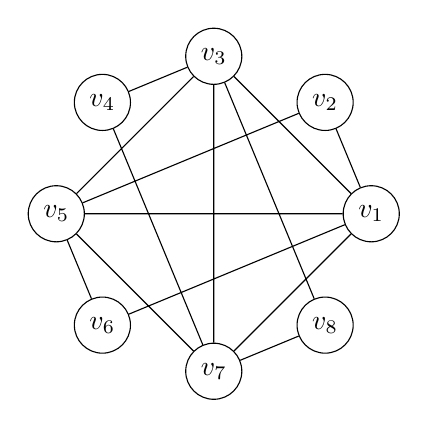
\begin{tikzpicture}[scale=2, bend angle=22.5]
\tikzstyle{every node}=[draw,shape=circle];
\foreach \i in {1,...,8}
{
\path (45*\i-45:1cm) node (v\i) {$v_\i$};
}
\draw
(v1) -- (v2) (v3) -- (v4) (v5) -- (v6) (v7) -- (v8)
(v1) -- (v3) (v3) -- (v5) (v5) -- (v7) (v7) -- (v1)
(v2) -- (v5) (v4) -- (v7) (v6) -- (v1) (v8) -- (v3)
(v1) -- (v5) (v3) -- (v7);
\end{tikzpicture}
\end{center}

Later we will have an introduction to \packagename{tikz} and \packagename{pgf}. If you are interested in it, please refer to the \structure{pgf manual} by \mintinline{shell}|texdoc tikz| or \mintinline{shell}|texdoc pgf|.

\end{frame}

\begin{frame}{Another example}

Binary tree:
\begin{center}
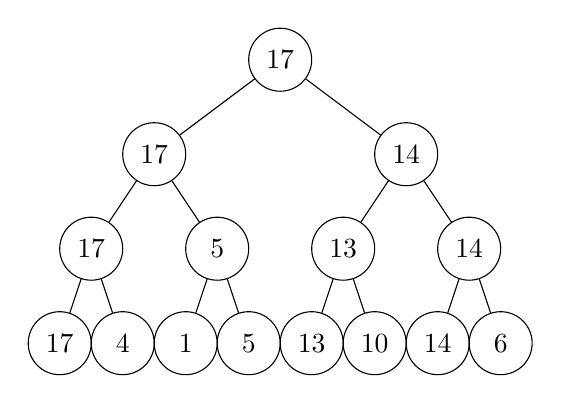
\begin{tikzpicture}[scale=0.8]
\tikzstyle{every node}=[draw,shape=circle,minimum size=0.8cm];
\node {17}[sibling distance=4cm]
child { node {17}[sibling distance=2cm]
	child {
		node {17}[sibling distance=1cm]
		child { node {17} }
		child { node {4} }
	}
	child {
		node {5}[sibling distance=1cm]
		child { node {1} }
		child { node {5} }
	}
}
child { node {14}[sibling distance=2cm]
	child {
		node {13}[sibling distance=1cm]
		child { node {13} }
		child { node {10} }
	}
	child {
		node {14}[sibling distance=1cm]
		child { node {14} }
		child { node {6} }
	}
};
\end{tikzpicture}
\end{center}

\end{frame}

\section{Tables}

\subsection{Tabulars}

\begin{frame}[fragile]{The \packagename{tabular} Environment}
	Table is another common element in \LaTeX, usually you will need the \packagename{booktabs, multirow} packages for enhanced functions of tables. You can insert the command in the preamble of your document.

\begin{command}
\LC|\usepackage{booktabs, multirow}|
\end{command}

\begin{latexexamplesplit}
\begin{tabular}{lcr}
  \toprule
  Title 1 & Title 2 & Title 3 \\
  \midrule
  1 & 2 & 3 \\
  \bottomrule
\end{tabular}
\end{latexexamplesplit}

The syntax is similar to the \packagename{align} environment in maths. \LC|&| is used to split the columns are \LC|\\| is used to split the rows.

\end{frame}

\begin{frame}{Warning}
  \begin{warning}
      Never, ever use vertical lines in tables.
      
      Never use double rules in tables.
  \end{warning}
  \medskip
  They are not professional!
  
  Please read \urllink{http://mirrors.ctan.org/macros/latex/contrib/booktabs/booktabs.pdf} for instructions on designing professional tables.
\end{frame}


\begin{frame}[fragile]{Column Format}

\begin{command}
\begin{LCL}
\begin{tabular}{format}
...
\end{tabular}
\end{LCL}
\end{command}

	\packagename{format} can be set as follow:
	\begin{itemize}
		\item \packagename{|} - vertical line (not recommended)
		\item \packagename{l} - align left in this column
		\item \packagename{c} - align center in this column
		\item \packagename{r} - align right in this column
	\end{itemize}
	\begin{example}
		\begin{minipage}{0.48\linewidth}
			\centering
			\packagename{lll} \medskip
			
        	\begin{tabular}{lll}
        		\toprule
        		Title 1 & Title 2 & Title 3 \\
        		\midrule
        		1 & 2 &3 \\
        		\bottomrule
        	\end{tabular}
		\end{minipage}
		\begin{minipage}{0.48\linewidth}
			\centering
			\packagename{c|cc} \medskip
			
        	\begin{tabular}{c|cc}
        		\toprule
        		Title 1 & Title 2 & Title 3 \\
        		\midrule
        		1 & 2 &3 \\
        		\bottomrule
        	\end{tabular}
		\end{minipage}
    \end{example}	
\end{frame}

\begin{frame}[fragile]{Combining Rows and Columns}

There are two commands being used to combine rows and columns
\begin{command}
\LC|\multicolumn{ncols}{format}{text}|

\begin{itemize}
	\item \packagename{ncols} - the number of columns to be merged
	\item \packagename{format} - the format of the merged column, excluding the left \packagename{|}
	\item \packagename{text} - the text in the merged column
\end{itemize}

\LC|\multirow{nrows}{width}[fixup]{text}|

\begin{itemize}
	\item \packagename{nrows} - the number of rows to be merged
	\item \packagename{width} - the width of the merged rows (use \packagename{*} for auto)
	\item \packagename{fixup} - the vertical position of the text (optional, default in the center)
	\item \packagename{text} - the text in the merged row
\end{itemize}	

\end{command}

To use the \LC|\multirow| command, you need to insert the package \packagename{multirow} in the preamble of your document.

\end{frame}

\begin{frame}[fragile]{Horizontal lines}
  There are four commands to create a horizontal line in a table.

  \begin{itemize}
    \item \LC|\toprule| - Top line
    \item \LC|\midrule| - Middle line
    \item \LC|\cmidrule{2-3}| - Middle line that you can choose the columns to be drawn
    \item \LC|\bottomrule| - Bottom line
  \end{itemize}
  \pause
  \begin{example}
    \begin{minted}{latex}
\begin{tabular}{ccccc}
  \toprule
  \multirow{4}{*}{Table} & Title 1 & Title 2 & Title 3 & Title 4 \\
  \cmidrule{2-5}
  & \multicolumn{2}{c}{Text 1} & 
  \multicolumn{2}{c}{\multirow{3}{*}{Text 3}} \\
  \cmidrule{2-3}
  & \multicolumn{2}{c}{Text 2} & \multicolumn{2}{c}{} \\
  \cmidrule{2-3}
  & Text 4 & Text 5 & \multicolumn{2}{c}{} \\
  \bottomrule
\end{tabular}
    \end{minted}
  \end{example}
\end{frame}

\begin{frame}[fragile]

\begin{latexexample}
\centering
\begin{tabular}{ccccc}
  \toprule
  \multirow{4}{*}{Table} & Title 1 & Title 2 & Title 3 & Title 4 \\
  \cmidrule{2-5}
  & \multicolumn{2}{c}{Text 1} & 
  \multicolumn{2}{c}{\multirow{3}{*}{Text 3}} \\
  \cmidrule{2-3}
  & \multicolumn{2}{c}{Text 2} & \multicolumn{2}{c}{} \\
  \cmidrule{2-3}
  & Text 4 & Text 5 & \multicolumn{2}{c}{} \\
  \bottomrule
\end{tabular}
\end{latexexample}
\medskip
Just leave blank in the rest rows of \LC|\multirow|.

\end{frame}


\begin{frame}[fragile]{Table Generators}
	With \LC|\multirow| and \LC|\multicolumn|, we can almost draw tables of any style, but this coding process can never be as easy as the graphic one, like making tables in Word or Excel. Is there any ways to convert graphic tables into \LaTeX\ codes directly?\\
	\begin{itemize}
		\item Use \LaTeX\ Table Generator: \url{http://www.tablesgenerator.com/}
		\item \LaTeX\ Complex Table Editor: \url{https://www.latex-tables.com/}
		\item Excel2latex: \url{https://ctan.org/tex-archive/support/excel2latex/}
	\end{itemize}
\end{frame}

\subsection{Tables}

\begin{frame}[fragile]{The \packagename{table} Environment}

The \packagename{table} environment is used to arrange the place of a tabular, similar to the \packagename{figure} environment. Here is a template of how to use the environment.

\begin{command}
\begin{LCL}
\begin{table}[position]
  \centering
  \caption{caption}
  \begin{tabular}{format}
    ...
  \end{tabular}
  \label{table:label}
\end{table}
\end{LCL}
\end{command}

The \packagename{position}, \packagename{caption}, \packagename{label} are same as those in the \packagename{figure} environment.
It's recommended to put the caption above the table.
\end{frame}

\begin{frame}[fragile]{Recall the Positions}
	We usually want to place the graphs or tables just below or above the content where we mention them, but even when we type \packagename{[h]} in position, you can not ensure that it will appear at the ideal position, and there are several methods to make up for this. You can try them one by one: \medskip
	\pause
	\begin{enumerate}[<+->]
		\item Change \packagename{[h]} to \packagename{[!h]}
		\item Change \packagename{[!h]} to \packagename{[!H]}
		\item Use \LC|\newpage| to move the following content to the next page
	\end{enumerate}\medskip
	\pause
Usually you don't need to pay too much attention about where the figures and tables are exactly are because you can use \LC|\ref| to reference them. And the numbering of 	figures and tables will strictly follow the order of their code.
	
\end{frame}
